\chapter{Parallel Programming and Performance}

	A short introduction to parallel programming and scalability will be given,along with the writers parallel implementation of FSS, a performance and scaling overview and a short comparison with WL.

\section{Parallel Programming}

	As the majority of modern CPUs have at least 4 physical processing cores, CPU code parallelization has become more important then ever to exploit all of the performance provided by modern CPUs. Not only that but as the problem that we are trying to solve becomes more complex or when we want to simulate bigger systems, single core computations may not be able to solve the problem in a reasonable amount of time. This way there is a need for parallelization. GPU computing is also an alternative but, generally, is a more complex approach.

%	A program is executed in a process. A process has its own code, data, memory space (stack and a heap), and other specific sets of data. Other processes do not have access to another process data or memory space. A process is executed in only one CPU core. Within a process there is at least one thread, meaning that a process can be single-threaded or multi-threaded. A thread is a sequence of code that is being executed. Each thread has its own stack, and data, however they share the data that is common to the main thread and the heap between them.

	In computer science there are two main paradigms for parallel applications \cite{Hager2011}. One based on threads, shared memory parallel programming, and another based on processes, distributed memory parallel programming. 
	A shared memory program is executed in multiple threads that coexist in the same memory space. Thus each one has access to the other memory and vice-versa. Therefore communication between concurrent executions of the code within the process is easy. However with multi-threading the code can only be executed in the same computer since it is only run in a single process. Multiple threads running within the same process can reduce parallel performance,. In C/C++, there are many libraries that implement this style of programming, such as OpenMP and PThreads. 
	On the other hand, a distributed memory concurrent program is executed through various processes each in their own memory space. Communication between processes is harder than thread communication. Multi process communication is more performance taxing since they live in different memory spaces. Excessive communication can lead to performance downfalls This downside, however, comes with better parallel performance and the ability to execute computations in various computing nodes. The default C/C++ library for distributed memory parallel programming is the message passing interface (MPI) having many implementations, such as OpenMPI, MPICH or MVAPICH.


\subsection{Parallel Scalability and Amdahl's Law}

	Consider a certain task that takes a time $T$ to be solved sequentially by one core. Using $N$ workers, ideally, it would only take $T / N$ to complete the task. This is called a speedup of $N$. Ideally, this division assumes that the task can be divided into $N$ pieces of equal complexity, that take the same amount of time to finish. In reality this is not true, the $N$ pieces could have little differences in complexity resulting in some workers having to wait for the other to finish. This is known as load imbalance and induces serialization in the computations.
	
	Let us now construct a model for scalability \cite{Hager2011}. Considering the overall problem size is $s + p = 1$, where $s$ is the nonparallelizable part and $p$ is the perfectly parallelizable part.In theory, we would want $s=0$ and $p=1$. In reality, there are many reasons for a nonvanishing serial part. There can be algorithmic limitations meaning that there might be operations that can not be performed in parallel, bottlenecks in the computer system, such as shared paths to memory between different cores, and communications overhead meaning that in order for workers to inter-communicate there must be some serialization. This last point is often the cause for poor parallel performance. 
		
	The serial wall time can be written as
\begin{equation}
	T_s = s + p,
\end{equation}	
while the wall time of solving the same problem with $N$ workers comes to
\begin{equation}
	T_p = s + \frac{p}{N}.
\end{equation}
This way, application speedup or parallel scalability can be define as the quotient of parallel and serial performance. Serial performance is the serial work done over time
\begin{equation}
	P_s = \frac{s+p}{T_s} = 1,
\end{equation} 
and parallel performance is
\begin{equation}
	P_p = \frac{p+s}{T_p} = \frac{1}{1-p+\frac{p}{N}}.
\end{equation}
The application speedup is now
\begin{equation}\label{eq:amd_law}
	S = \frac{P_p}{P_s} = \frac{1}{1-p+\frac{p}{N}}.
\end{equation}

\begin{figure}[h]
	\centering
	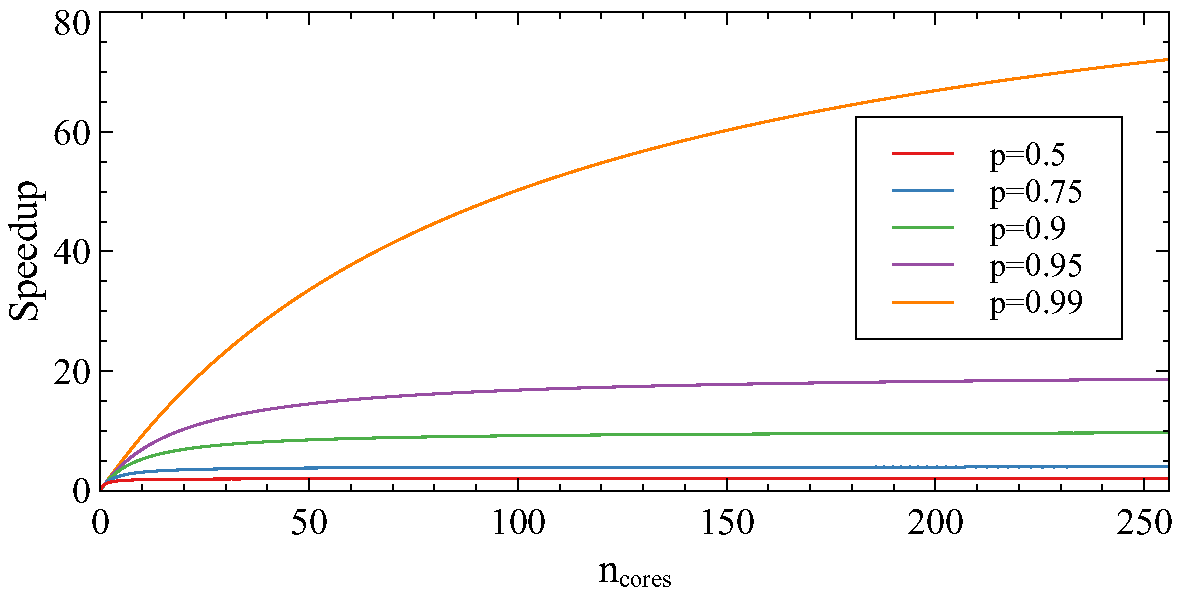
\includegraphics[scale=0.45]{performance/speedup_03.pdf}
	\caption{Speedup from Amdahl's Law as a function of the number of cores for five different values of the parallel portion of the code $p$.}
	\label{amd_law}
\end{figure}

Equation \ref{eq:amd_law} is known as Amdahl's Law, derived by Gene Amdhal in 1967 \cite{Amdahl1967}. This limits the speeup when $N \rightarrow \infty$ to $1/(1-p)$. This famous equations tells us how much faster can a program run when using $N$ CPU cores. In Figure \ref{amd_law} the Amdahl's Law speedup is plotted against the number of cores for different values of $p$.

	There are modifications to this law \cite{On2014} to accommodate system bottlenecks, parallel synchronization and inter-core communications. The most noteworthy is the Hill and Marty's model \cite{Hill2008}, which introduces a new way of defining the work and performance. An asymmetric architecture has one manager that does not work and a symmetric architecture has a manager that also does work. The performance of the Hill and Marty's model depends on the type of architecture considered. 
\begin{equation}
		P(N, r) = \twopartdef { \frac{N-r}{r} \sqrt{r} } {\text{symmetric}} {n-r} {\text{assymetric}}
\end{equation}
where $r$ is the size of the sequential core used during the parallel execution. 


\section{Implementation}

	Due to the nature of FSS algorithm we can have various independent walkers sampling their own histogram. Each walker performs an independent random walk with access to the whole energy space and constructs a histogram for a magnetization $M_q$. All of the sampled histograms are combined to compute the DoS at $M_{q+1}$. The next iteration is performed using the computed DoS by joining all of the histogram contributions in the last iteration.
This way, in one iteration there is only need for 2 communications, one is the broadcasting of the computed DoS in the last iteration to all of the walkers, the other is the collection of the sampled histograms by all of the walkers. There is a need for one walker to execute all of the serial computations such as the outputting to the terminal and to files, and joining all of the DoS at the end of an iteration and broadcasting it to all of the other walkers. Considering this approach, distributed memory parallelism was the better option for a high performance implementation and MPI was used to carry the process to process communications.
	
	The MPI implementation starts by assigning each walker a different seed for the RNG, so the results come from different streams of random numbers. This is achieved by multiplying a defined seed by the number assigned to that walker. Then, the first iteration is computed by the manager process and broadcasted to all of the walkers. When all of the walkers have sampled the assigned number of configurations, they send the histogram to the manager and it computes the DoS at the third magnetization finally broadcasts it to the walkers. This is repeated until $q = q_{max}$. At the end, the manager writes the output files. As the only serial operations is the output to the terminal and the normalization of the JDoS at the end of an iteration we can expect a close to linear parallel scalability.

%	There are two ways of dividing the computations between $n$ walkers. Each performs a random walk with $\text{REP}_{walker} = \text{REP} / n$ giving us the wall time of a single core computation with REP samples per energy divided by the number of walkers or having each walker sample REP configurations per energy giving us the wall time of a single core REP computation. 
 
	Two scenarios of this implementation were explored. One where the manager also performed is own random walk through the energy space, acting like a manager and a walker, and another were the manager only performed the single core operations.Here the advantage is on the side of the first scenario, since there is one more walker and having that walker also performing single core tasks gives an overall better performance than having one idle processes during 95\% of the computation.
\pagebreak

\section{Method Performance}

	Now let us discuss the performance of FSS method of both implementations starting by the single core performance and moving on to scaling tests. The following single core benchmarks were performed in a computer equipped with a Ryzen 9 5950X at stock speeds.  
	
	In Figure \ref{L4_wall_time}, we can observe the wall time and the time spent sampling per energy value as a function of the parameter REP. We can see as we increase REP by 10x, the wall time is also increased by 10x.
	
\begin{figure}[ht]
\centering
\subfigure[]{%
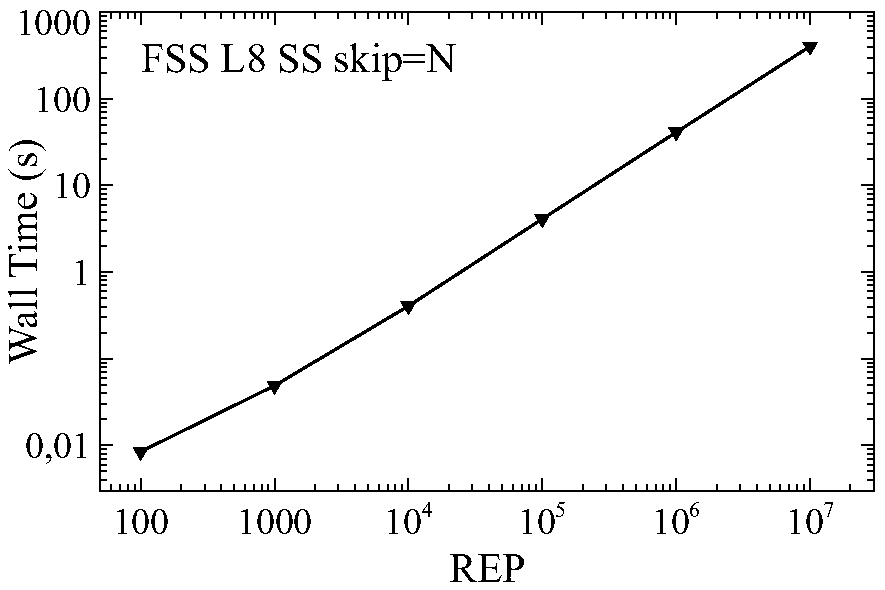
\includegraphics[scale=0.4]{performance/speedup_01.pdf}
\label{L4_wall_time}}
\quad
\quad
\quad
\subfigure[]{%
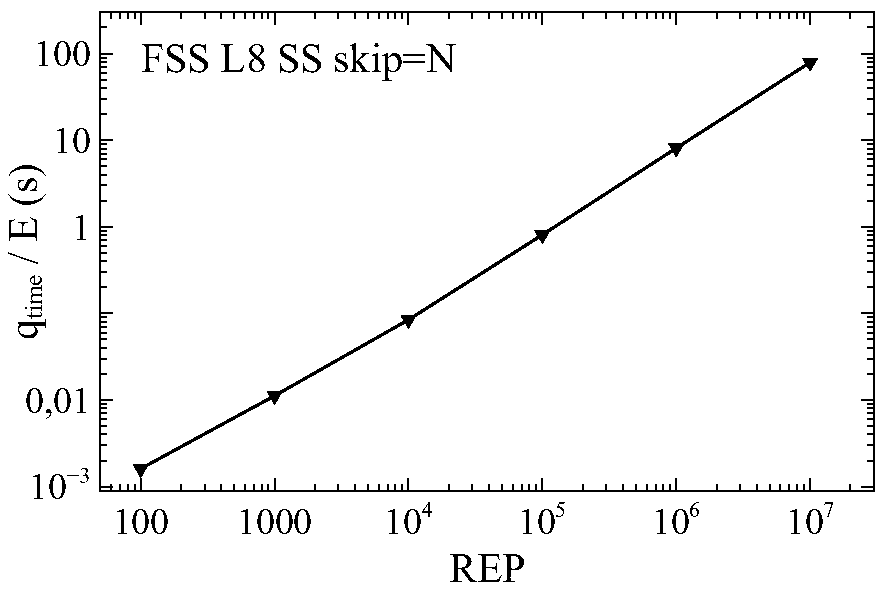
\includegraphics[scale=0.4]{performance/speedup_02.pdf}
\label{L4_q_time}}	

\caption{(a) LogLog plot of the single core wall time of FSS as a function of the number of samples per each energy point, REP.  (b) LogLog plot of the time spent sampling for each energy value, $q_{time}/E$.These are computations for a system with 16 spins. Data was averaged over 1000 computations to reduce statistical error.}
\label{wall_time_L4}
\end{figure}

	The time spent sampling configurations for each energy value, $q_{time}/E$, is a very important metric, Figure \ref{L4_q_time}. This value is computed by dividing the wall time spent on that iteration by the number of sampled energy points. Each iteration of the simulation we should be attentive to the behaviour of $q_{time}/E$, since it can tell us if the computations are stable or the number of samples, REP, must be increased. 
For a stable calculation, this time must remain approximately the same throughout the computation. If $q_{time}/E$ keeps increasing each iteration then the value of REP is insufficient to correctly explore the energy space for a given magnetization. This causes the JDoS estimate to be less accurate or in the worse cases to be wrong.The obvious solution would be to increase the value of REP, but increasing the skip value can be enough in some cases.

	The FSS method scales linearly with the repetitions,Figure \ref{wall_time_L4}, so given the wall time of that system with a certain REP value we can easily estimate how much time the computations will take for a another REP value.
When running the algorithm for a new system we can not have a precise estimation for the wall time. However, knowing only the $q_{time}/E$ for the first iterations and assuming that the REP value is sufficient so that this time does not increase, we can estimate the full wall time to estimate the complete JDOS. Assume that the system has $NE$ values of energy and $NM$ values of magnetizations available.The JDoS will have $NE \times NM$ points, but since we only compute half of the JDoS, $( NE \times NM ) / 2$. Considering the typical shape of the (E,M) phase space of the Ising model, about $1/3$ to $1/2$ of those points will be different than 0, so the estimation for the wall time comes as 
\begin{equation}\label{estimation}
	\text{Wall Time} \approx (q_{time}/E) \frac{NE \times NM}{2} \times \text{fraction of non-zero points} .
\end{equation}

\pagebreak

\begin{table}[h]
\centering
\caption{Wall Time of some Ising systems with their respective wall time estimates by Equation \ref{estimation} with two different values for the fraction of non-zero energy points.} 
\begin{tabular}{c|c|c|c|c|c|c}
Lattice & $N$   & $NE \times NM$ & $q_{time}/E$ & Wall Time & Estimate $1/3$ & Estimate $1/2$ \\ \hline
SS      & $16$  & $289$                         & $0.11s $        & $4s$        &$ 5s$                  & $8s$                  \\
SS      & $64$  & $4225$                        & $0.85s$         & $728s$      & $600s $               & $900s    $ \\
SS      & $256$ & $66049$                       & $1s$            & $18942s$    & $10898s $             & $16512s  $ \\
SC      & $64$  & $6305$                        & $1.1s $         & $1148s$     & $1144s$              & $1733s $           \\
FCC     & $256$ & $197633$                      & $20s$           &$ 871118s$   & $652188s$      & $988165s$            
\end{tabular}
\label{wall_time_table}
\end{table}

	Table \ref{wall_time_table} presents different wall times for single core computations and their respective estimation through Equation \ref{estimation} for two different fractions of non-zero energy points, $1/3$ and $1/2$. For larger Ising systems in 3D lattices, computation times can get very large. As we will see in the next Section, we can greatly reduce them through parallelism. 


\subsection{Parallel Scaling}
	
	The tests for parallel scaling were performed on the Cirrus-A computing cluster on INCD facilities under the Advanced Computing Projects grant, reference CPCA/A1/7252/2020 with support from FCT. In this project tests with a maximum of 320 cores were performed to better understand the parallel scalability of the Flat Scan Sampling method.

	Having constructed a model for parallel scalability, Equation \ref{amd_law}, we can fit Amdahl's Law to experimental wall time values as a function of the number of cores $n$. For this we need to solve Equation \ref{amd_law} for $p$ since our interest is to gain an insight about the portion of the algorithm that is perfectly parallelized.
\begin{equation}
	p_n = \frac{n}{n-1} \left( 1 - \frac{1}{S(n)} \right),
\end{equation}
where $S(n) = T_1 / T_n$. The mean value of $p$ is then
\begin{equation}
	p = \frac{1}{N-1} \sum_{i=2}^{N} p_i.
\end{equation}
This is the standard method to estimate $p$ given the wall time per number of cores. Through this method we find  $p=0.9655\approx 0.97$, blue line in Figure \ref{amd_fits}.

\begin{figure}[h]
	\centering
	\subfigure[]{
	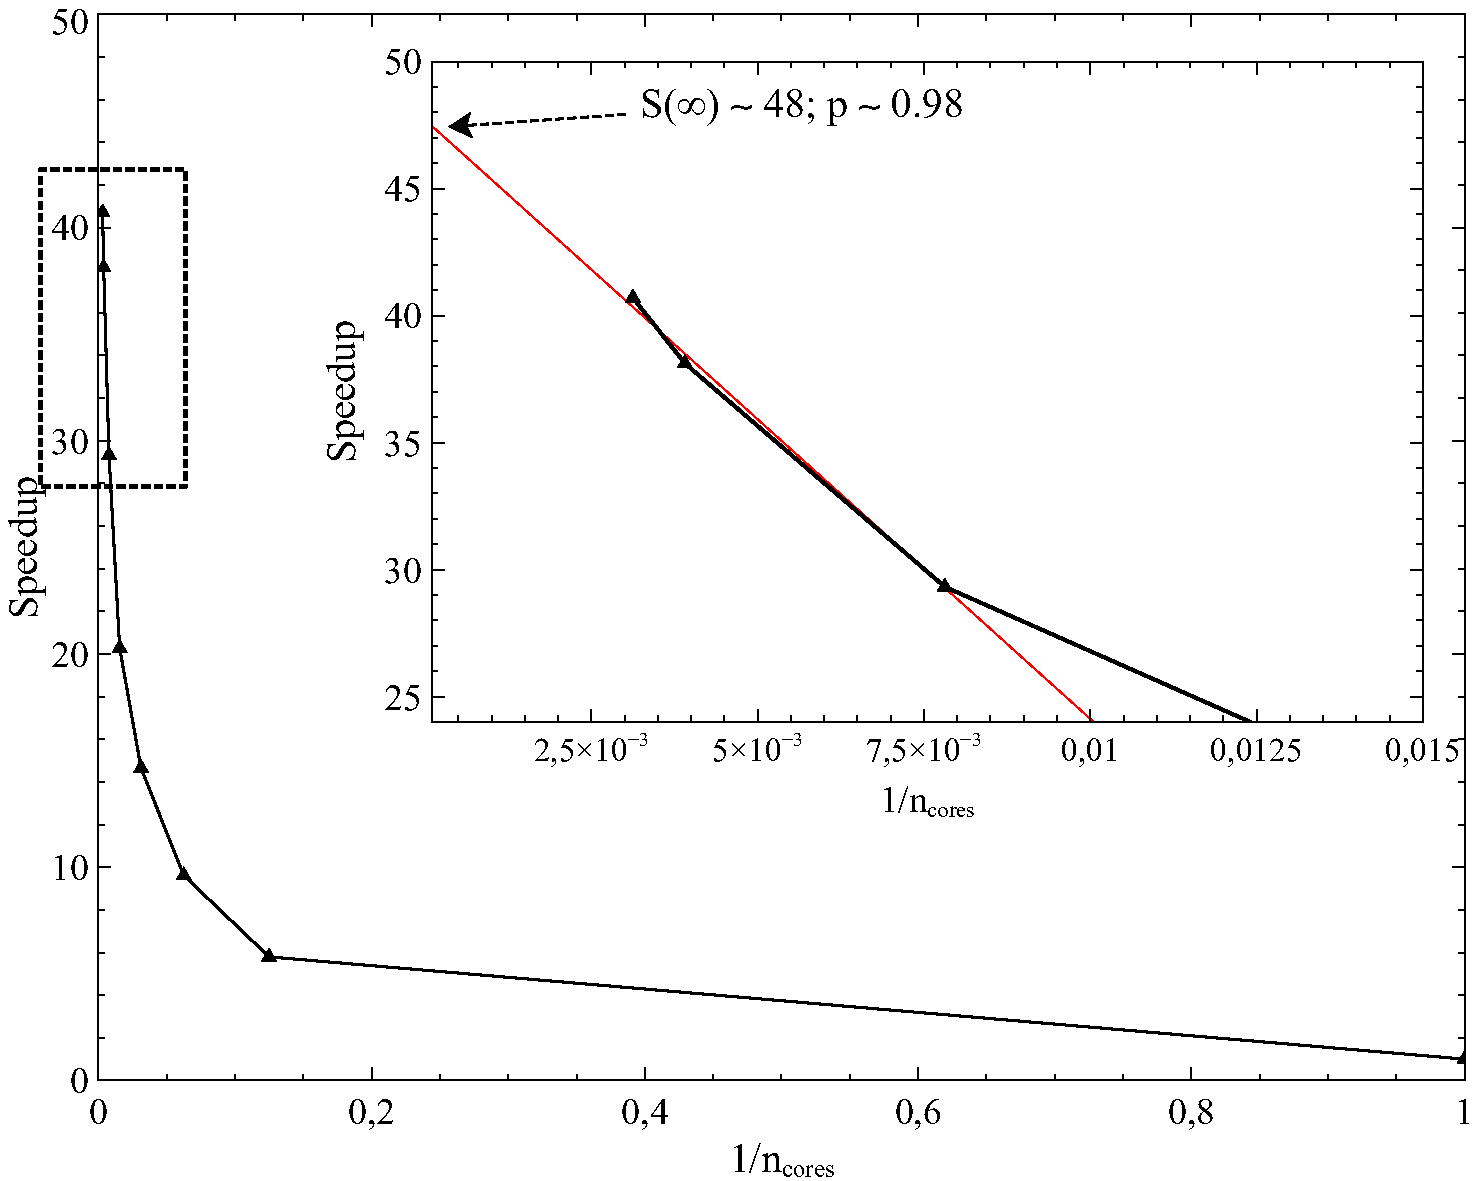
\includegraphics[scale=0.29]{performance/speedup_04.pdf}
	\label{inf_S}
	}
	\subfigure[]{
	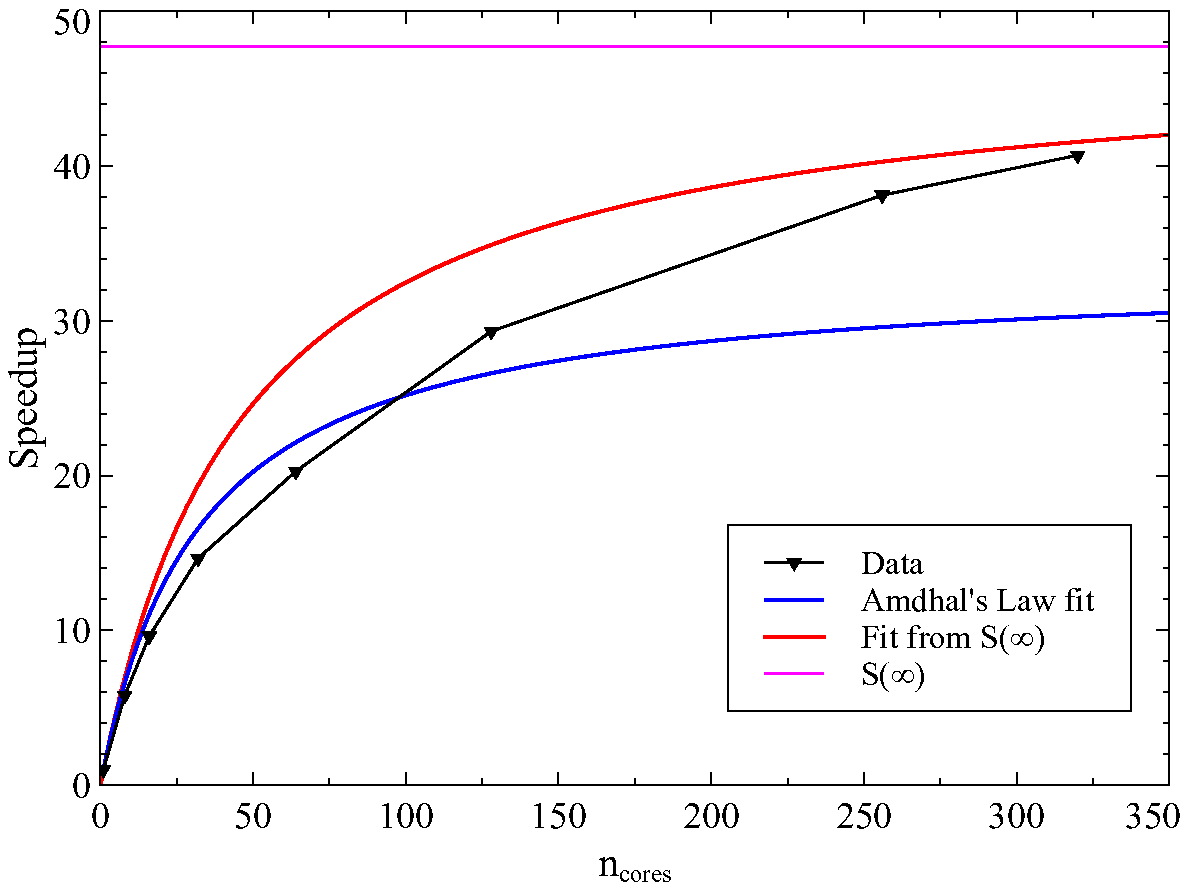
\includegraphics[scale=0.38]{performance/speedup_05.pdf}
	\label{amd_fits}
	}
	\caption{(a) Extrapolation of the speedup for an infinite number of cores. We have a limiting speedup of 48 and an $p \approx 0.98$ (b) Amdahl's law fitted for the wall time data. The fit from Amdahl's Law and from the speedup at infinite cores create a lower and upper bound, respectively.}
\end{figure}

%\pagebreak

	Another method to estimate $p$ is to find the speedup for and infinite number of cores $S(\infty)$ and by using the relation
\begin{equation}
	S(\infty) = \frac{1}{1-p},
\end{equation}
we can estimate $p$. The best way to find the speedup of infinite cores is to plot $S(1/n)$ and perform a linear extrapolation for $1/n=0$, Figure \ref{inf_S}.Here we obtain a limiting speedup of 48 and a value for $p$ of 0.98, very close to the valued found by the standard method.

	In Figure \ref{amd_fits}, the Amdahl's Law curves for the two values of $p$ estimated are shown along with the experimental data from the cluster. Neither of the methods of estimating $p$ give accurate results, since in our model we are not considering communications overhead nor architectural constrains. A more in depth and accurate study could be done, considering for example the Hill and Marty's model \cite{Hill2008}.  

	However some strong conclusions can still be drawn.The standard method for estimating $p$ acts as a lower bound for the speedup while the $S(\infty)$ method acts as an upper bound, since the experimental data is bounded by these two fits. We have found that $0.97<p<0.98$. This is a remarkable result, since it means that 97 to 98\% of the algorithm can be perfectly parallelized. In other words, if we split the between $N$ walkers, 98\% of the single core wall time will be divided by the $N$ walkers. Thus we can conclude that Flat Scan Sampling is a highly parallelizable algorithm and can have performance gains upto 48 times the single core wall time.

\section{Comparison with Wang-Landau - Performance}

	In the previous Chapter we have already look at the differences in precision and accuracy between Flat Scan Sampling and Wang Landau. Now a comparison of the performance will be given. In this Section will use the same L8 SS results from the last comparison Section.
		
\begin{figure}[h]
	\centering
	\subfigure[]{
	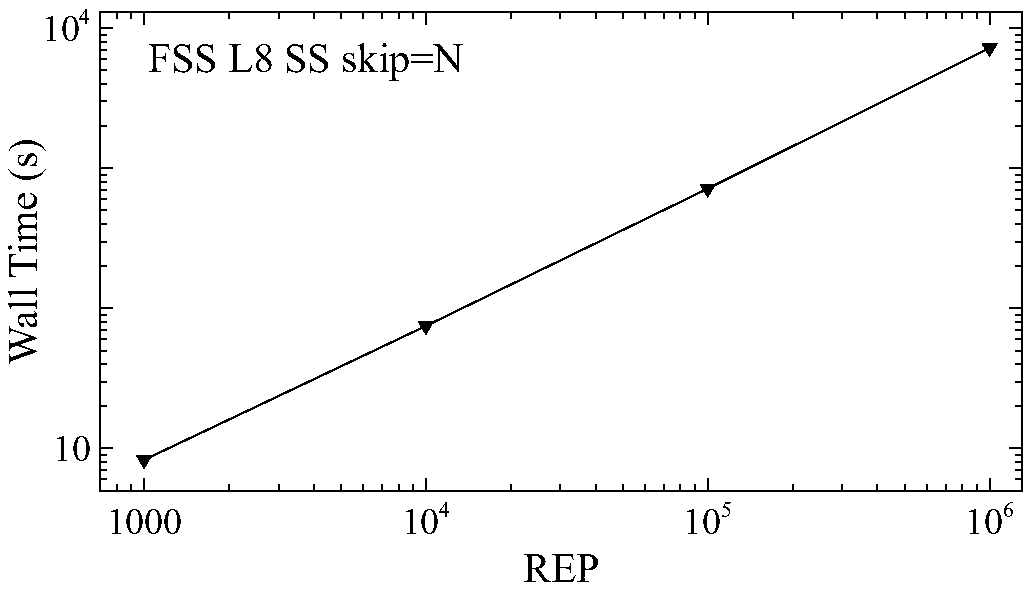
\includegraphics[scale=0.4]{comparison/wl_comp_01.pdf}
	\label{fss_time}
	}
	\subfigure[]{
	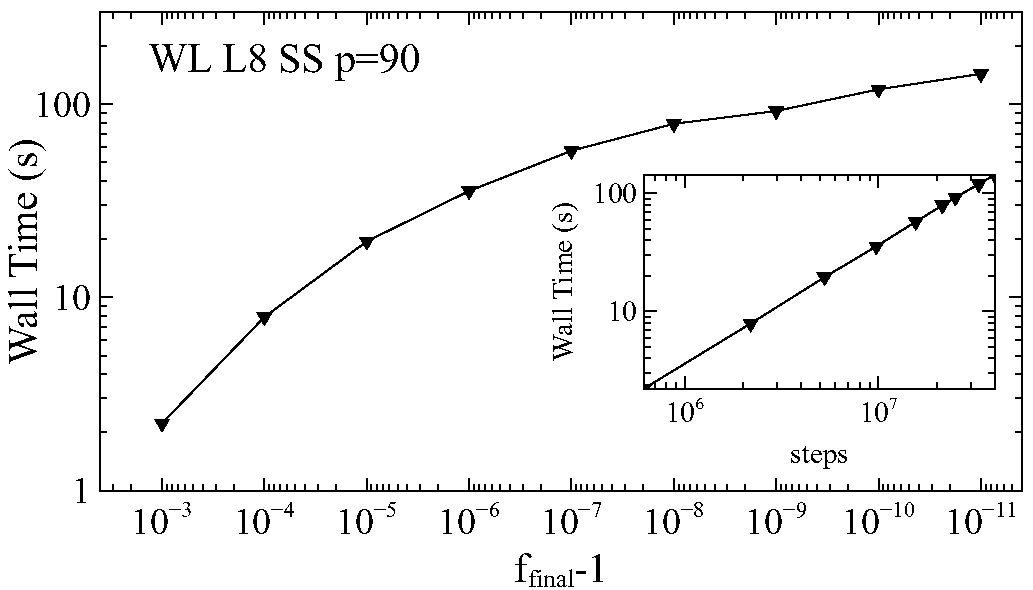
\includegraphics[scale=0.4]{comparison/wl_comp_02.pdf}
	\label{wl_time}
	}
	\caption{Wall time in seconds as a function of REP for FSS (a) and as a function of $f_{final}$ and the steps taken during the simulation for WL sampling (b).}
\end{figure}

	The single core wall time of FSS scales linearly with the parameter REP, Figure \ref{fss_time}, however for the WL sampling, the wall time is not linear with the parameter $f_{final}$. Our interest in this Section is to study the performance of WL as a function of the steps in the simulation. In the inset of Figure \ref{wl_time} we can see that WL also scales linearly with the steps in the simulation.
	
	One important point to highlight is that the wall time of FSS is very predictable as shown in Table \ref{wall_time_table}. The wall time of WL sampling can not be that easily predicted. Due to the real time estimation of the JDoS, Wang-Landau's random walk is very unforeseeable and it can get stranded, for a while, between a few points in the phase space, wasting a lot of time, Figure 4 and 5 in \cite{Nguyen2006}. Thus we can have faster than average simulations or very long simulations. 
	On the other hand, we have seen if the value of REP is not high enough, Flat Scan Sample's random walk can get stuck and never finish. With Wang-Landau we are assured that the computation will always finish, even if it takes a very long time.

	A critical advantage of Flat Scan Sampling is the power of parallelization. Since FSS is an embarrassingly parallel algorithm and, if well implemented and optimized, $0.97<p<0.98$, Figure \ref{amd_fits}, we can achieve parallelization with up to 48 times performance gains. This also means that a GPU implementation is easily in reach. Although it is possible to parallelize the Wang-Landau algorithm, it is much harder than FSS, since we have to divide the phase space between different walkers and have them communicate at the barriers \cite{Yin2012}.

\begin{figure}[h]
	\centering
	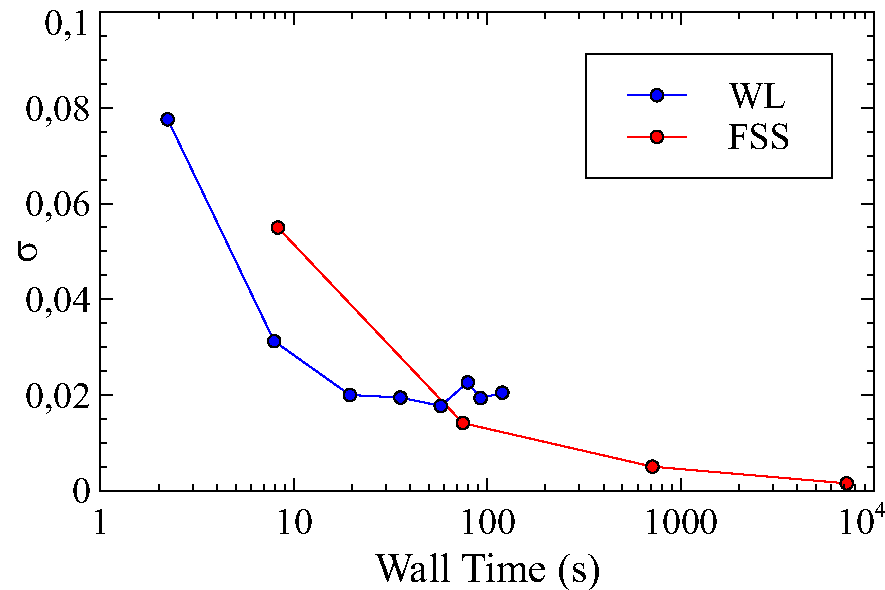
\includegraphics[scale=0.5]{comparison/wl_comp_05.pdf}
	\caption{Standard deviation as a function of the wall time for the Checker Board configuration for an L8 SS Ising system.}
	\label{time_std}
\end{figure}

	To finalize this comparison, let us shift our focus to Figure \ref{time_std}. Here we can see the standard deviation as a function of wall time for the FSS and the WL method for two flatness conditions. For the Wang-Landau with $p=90$, we can get a more precise solution with Flat Scan Sampling int the same or less computing time with REP$\ =10^4$ (second point).In order to get a more refined solution with WL sampling, we need to increase the flatness condition, green line in Figure \ref{time_std}. Flat Scan Sampling still has more precision with less or equal computing time with a value of REP between $10^4$ and $10^5$. Therefore,  we can conclude that FSS will have better precision in the calculations per computing time than the WL method.

	Having done this comparison we can take a few important and string conclusions. Flat Scan Sampling and Wang-Landau method are two vastly different methods. FSS can be as accurate at the cost of computing time, while WL's accuracy and precision plateaus for all flatness criteria.WL's precision per simulation time is worse in most cases than FSS's. Thus, FSS is a better method to obtain fairly quick and very precise computations while with WL we can get an inaccurate solution very quickly.









